\documentclass{beamer}

\usepackage{xltxtra}
\usepackage[lithuanian]{babel}
\usepackage{mathtools}
\usepackage{cite}
\usepackage{multimedia}

\title{Difuzijos įtakos krūvininkų pernašai ir rekombinacijai skaičiavimas}

\author
{V. Valentinavičius}

\date{Vilnius, 2012}
\subject{Kursinis darbas}

\begin{document}
\frame{\titlepage}
  \begin{frame}
    \frametitle{Darbo tikslai}
    \begin{itemize}
      \item Naudojant skaitmeninį modeliavimą nustatyti eksperimentines sąlygas, kurioms esant negalima atmesti difuzijos įtakos rezultatams gautiems naudojant fotogeneruotų krūvininkų ištraukimo tiesiškai kylančia įtampa (photo-CELIV) metodiką.
	\item Naudojant skaitmeninį modeliavimą pademonstruoti ir paaiškinti difuzijos įtaką rekombinacijos koeficiento matavimams.
	\item Naudojant skaitmeninį modeliavimą patikrinti krūvininkų judrio skaičiavimų rezultatų validumą.
    \end{itemize}
  \end{frame}
  \begin{frame}
    \frametitle{Photo-CELIV}
    \begin{figure}
    	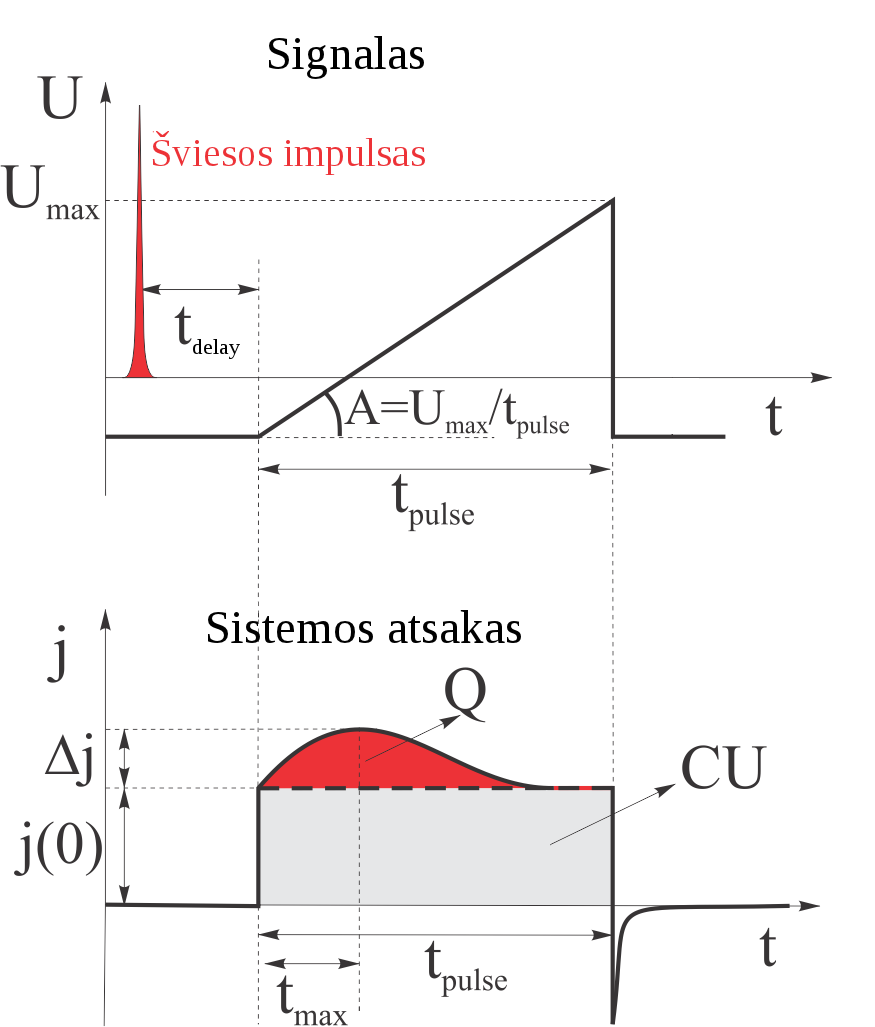
\includegraphics[height=0.8\textheight]{./media/celivTransients.png}
    \end{figure}
  \end{frame}
  \begin{frame}
    \frametitle{Priemonės}
    \begin{itemize}
	\item Naudota autoriaus sukurta programa skirta spręsti krūvininkų pasiskirstymo uždavinius
	\item Programa leidžia atkartoti realaus eksperimento eigą ir sąlygas 
	\item Tirtas virtualaus bandinio elgesys simuliuojant photo-CELIV metodiką
	\end{itemize}        
  \end{frame}
  \begin{frame}
  	\frametitle{Analizuotos metodikos}
  	\begin{itemize}
  	\item Krūvininkų rekombinacijos įvertinimas pagal photo-CELIV kinetikų maksimumo soties vertę
  	\item Krūvininkų judrio skaičiavimas pagal photo-CELIV kinetikų maksimumo padėtį
  	\end{itemize}
  \end{frame}
  \begin{frame}
    \frametitle{Parametrai}
    \begin{itemize}
	\item Krūvininkų judrių santykis \(\frac{\mu_n}{\mu_p} = 1000\)
	\item Bimolekulinė rekombinacija pagal Lanževeną \(B_L=\frac{e}{\varepsilon \varepsilon_0}(\mu_n+\mu_p)\)
	\item Difuzijos koeficientas suskaičiuojamas pagal Einšteino sąryšį \(D=\frac{k_B T \mu }{e}\)
	\end{itemize}
  \end{frame}

  \begin{frame}
    \frametitle{Svarbiausi darbo rezultatai ir išvados}
    \framesubtitle{Difuzijos įtaka photo-CELIV srovės sotinimuisi}
    \begin{figure}
    	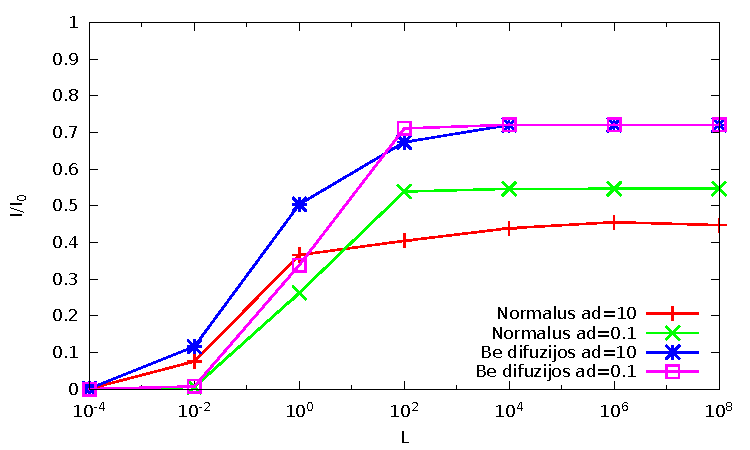
\includegraphics[width=0.9\textwidth]{./media/pdf/semilogsaturation.pdf}
    \end{figure}
    \begin{itemize}
    \item Photo-CELIV srovės kinetikos maksimumo vertės sotinimasis nuo šviesos intensyvumo parametro
    \end{itemize}
  \end{frame}
    
  \begin{frame}
    \frametitle{Svarbiausi darbo rezultatai ir išvados}
    \framesubtitle{Difuzijos įtaka photo-CELIV srovės sotinimuisi}
    \begin{itemize}
		\item Difuzija padidina išmatuotą rekombinacijos koeficientą bandinyje, jei matavimui naudojama photo-CELIV srovės kinetikos soties vertė. Pokytis gali siekti 20-50\% priklausomai nuo krūvininkų sugerties profilio.
    \end{itemize}
  \end{frame}
  
  \begin{frame}
    \frametitle{Svarbiausi darbo rezultatai ir išvados}
    \framesubtitle{Difuzijos įtaka judrio vertės skaičiavimui}
    \begin{figure}
    	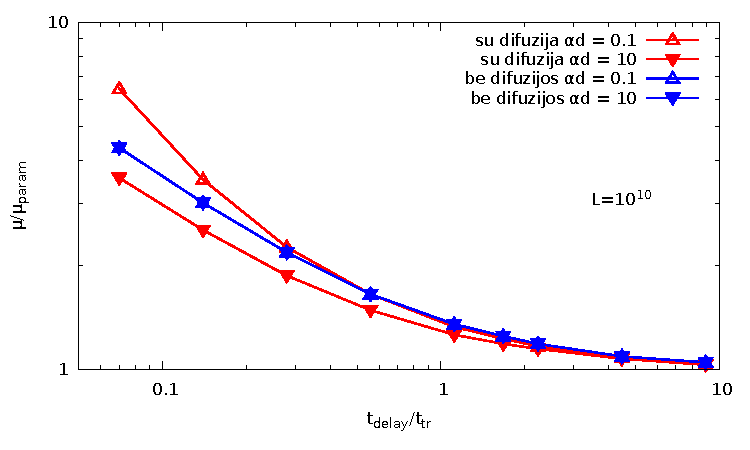
\includegraphics[width=0.9\textwidth]{./media/pdf/log_mobility.pdf}
    \end{figure}
    \begin{itemize}
    \item Pagal photo-CELIV srovės kinetikų maksimumo padėtis suskaičiuoto judrio priklausomybė nuo simuliacijos parametrų
    \end{itemize}
  \end{frame}

  \begin{frame}
    \frametitle{Svarbiausi darbo rezultatai ir išvados}
    \framesubtitle{Difuzijos įtaka judrio vertės skaičiavimui}
    \begin{itemize}
      \item Krūvininkų judrio matavimo rezultatai iš photo-CELIV kinetikos maksimumo padėties priklauso nuo užlaikymo trukmės. Tai lemia pradinis krūvininkų kiekio kitimas dėl rekombinacijos.
      \item Įskaičius difuziją, esant $t_{delay} < t_{tr}$ judrio vertė papildomai pakinta iki 2 kartų, priklausomai nuo pradinio pasiskirstymo. Difuzija pakeičia krūvininkų pasiskirstymo pavidalą.
    \end{itemize}
  \end{frame}
  
  \begin{frame}
  \frametitle{Pabaiga}
  Gal turite klausimų?
  \end{frame}
  
\end{document}